\chapter{Evaluation}

In this chapter we will show some experiment results of our system. We will use various applications which will cover all the aspects of our implementation includes thread interleaving synchronization, application instrumentation and system call synchronization. With all the evaluation, we will answer the following questions:

\begin{itemize}
  \item Correctness: Given the same input, can the primary and secondary consistently generate the same output?
  \item Performance: Compare to non-replicated execution, how much overhead is introduced by our system?
  \item Breakdown: Where does the overhead come from?
\end{itemize}
% Evaluation factors:
% 1. Lock count & pcnmsg count for schedule part
% 2. Breakdown
% 3. Absolute time

\paragraph{Evaluation Setup} All experiments were run on a server machine with 4 AMD Opteron 6376 Processors (16 cores each, 2.3Ghz), which is 64 cores in total. The total RAM is 128GB. Our Popcorn Linux kernel was installed on Ubuntu 12.04 LTS. We partitioned the hardware resources into half, one for the primary and one for the secondary. Each of them has the full control of their own 32 cores and 64GB RAM. The machine comes with a 1Gbps high speed connection. For benchmarking server applications, we used a machine in the same rack, connected to the same switch, to act as the benchmark client.

\section{Racey}
We used a variant of racey~\cite{hillstress} to evaluate the correctness of our system. racey benchmark is a set of concurrent programs which read and write some shared data concurrently with various concurrent models. With a non-deterministic system, all the benchmark will create a different result during each different run. We use racey to validate if we can have the same thread interleaving on primary and secondary, which should lead the same output on both primary and secondary.

\paragraph{racey-guarded} racey-guarded has a global array, it uses pthread to create multiple threads and modify the global array concurrently. The access to the global array is protected by pthread\_mutex\_lock. We tested this one without any modification to the application. With both synchronization algorithms, we are able to create consistent results on the primary and secondary for over 100 consecutive runs.

\paragraph{racey-forkmmap} racey-forkmmap utilizes mmap to create a shared memory area, and uses fork to create multiple processes to read and modify the shared memory area. We manually added \_\_det\_start and \_\_det\_end around each access to the shared memory area. With both synchronization algorithms, we are able to create consistent results on the primary and secondary for over 100 consecutive runs.

\paragraph{racey-tcp} Based on the idea of racey, we developed racey-tcp to stress the determinism for I/O related tasks. racey-tcp uses pthread to create multiple threads. One thread listens to the socket, whenever a new connection arrives, it puts the connection into a queue, other threads retrieve the connection from the queue, read the data on that connection and write the data into a file. For this benchmark, we wrapped the write system call for writing to the file with \_\_det\_start and \_\_det\_end. With both synchronization algorithms, we are able to create consistent output file on the primary and secondary for over 2000 requests.

\section{PBZip2}
% 1. threading model
% 2. A table of lock and cond var count
% 3. A table of instrumented dettick count
PBZip2 is the parallel version of bzip2. The concurrent model of this application is a typical producer-consumer model

% The concurrent model is shown in Figure~\ref{f:pbzip_model}. The FileReader thread reads the content of the file, break the input data into data chunks and put all the chunks into a queue. Worker threads get the data chunks from the queue 


%\begin{figure}
%\centering
%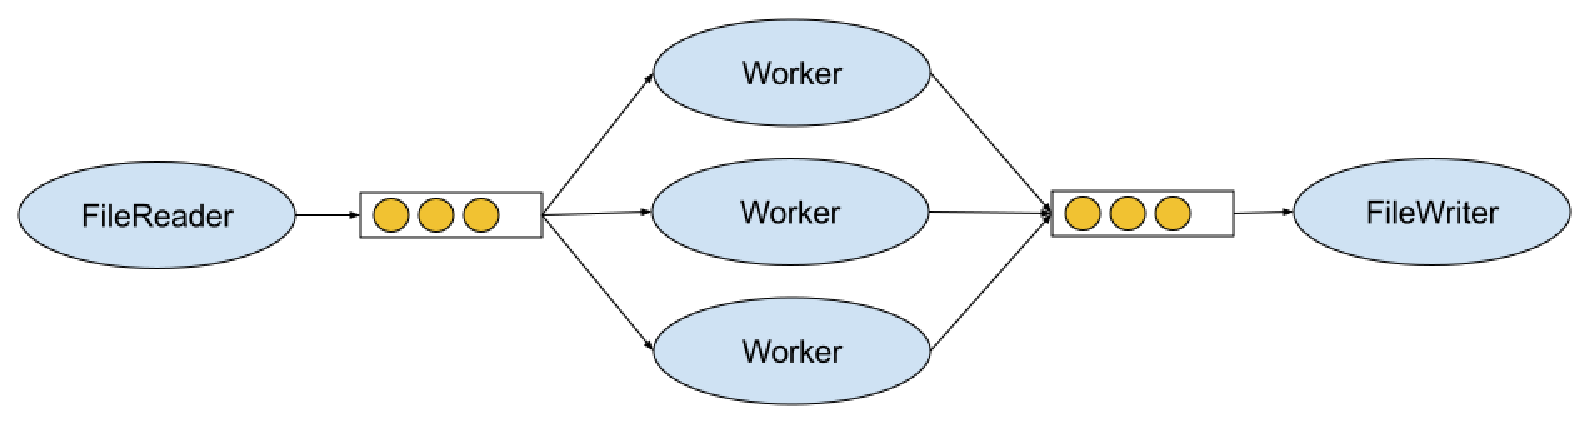
\includegraphics[width=0.8\columnwidth]{figures/pbzip2_model}
%\caption{pbzip2 concurrent model}
%\label{f:pbzip_model}
%\end{figure}

% instrumentation taken with what block size
% Benchmarks with certain block sizes

For PBZip2, the time consuming part is the place where it calls the libz2 compression/decompression functions. In this benchmark, we utilized the execution time profiling instrumentation to gain a decent performance in the deterministic execution, while for schedule replication nothing is modified.

Table~\ref{t:pbzip2_syscall} shows the system calls that are used by pbzip2, we only show the system calls that are tracked and synchronized by our system. In pbzip2,  gettimeofday is only used for showing the time spent on the whole process, so it is not critical to the output of the application. But since we synchronized it, both the primary and secondary showed the same finishing time all the time.

\begin{table}
 \caption{Tracked system calls used by pbzip2}
\begin{center}
 \begin{tabular}{c | c}
 System Call & Use in the Application\\ \hline
 gettimeofday & Calculate execution time
 \end{tabular}
\end{center}
\label{t:pbzip2_syscall}
\end{table}

\section{Mongoose Webserver}
% 1. threading model
% 2. A table of lock and cond var count

Mongoose is a compact multithreaded webserver.

Table~\ref{t:mongoose_syscall} shows the system calls that are used by mongoose. In mongoose, both system calls are critical to the final output.

\begin{table}
\caption{Tracked system calls used by mongoose}
\begin{center}
 \begin{tabular}{c | c}
System Call & Use in the Application\\ \hline
 time & Generate HTTP header  \\ \hline
 poll & Wait for accept, read and write
 \end{tabular}
\end{center}
\label{t:mongoose_syscall}
\end{table}

% show the performance of each thread count, then put the overall scalability.

\section{Nginx Webserver}
Nginx is a sophisticated webserver with multiple concurrent modes.

\begin{table}
\caption{Tracked system calls used by nginx}
\begin{center}
 \begin{tabular}{c | c | c}
System Call & Use in the Application\\ \hline
 time & Generate HTTP header\\ \hline
 poll & Wait for accept, read and write
 \end{tabular}
\end{center}
\label{t:nginx_syscall}
\end{table}


\section{Redis Database Server}
Redis is an in-memory database server. It uses a single thread to process requests, but it dynamically creates new threads to write the in-memory data to the disk. This benchmark is perfect for stressing the flexibility of dealing with dynamically spawned threads.

\subsection{Overhead Profiling}
\subsection{Results}
